\documentclass[11pt]{article}
\usepackage[margin=0.8in]{geometry}
\usepackage{amsmath}
\usepackage[boxed]{algorithm2e}
\usepackage[dvipsnames]{xcolor}
\usepackage{graphicx}
\usepackage{algorithm}
\usepackage{algorithmic}
\usepackage{hyperref}
\usepackage{mathtools}
\usepackage{tikz,graphics,color,fullpage,float,epsf,caption,subcaption}
\DeclarePairedDelimiter{\floor}{\lfloor}{\rfloor}
​
​
\title{CS3510-A: Design and Analysis of Algorithms, Spring 2021} 
​
\author{Homework-4}
​
\begin{document}
% \maketitle
\begin{center}
    
    \LARGE CS3510-A: Design and Analysis of Algorithms, Spring 2021 \\ \vspace{1em} 
    \large Homework-4 \\ \vspace{0.5em}
    February 9, 2021
\end{center}
\thispagestyle{empty}
\pagestyle{empty}
​
\noindent
\begin{center}
{\bf DUE DATE: Tuesday, February 16, 1l:59pm}
\end{center}
​
\noindent
{\bf Note-1:} Your homework solutions should be electronically formatted as a single PDF document that you will upload on Gradescope. 
If you have to include some handwritten parts, please make sure that they are very clearly written and that you include them as high resolution images. \\
​
\noindent
{\bf Note-2:} Please think twice before you copy a solution from another student or resource (book, web site, etc). 
It is not worth the risk and embarrassment. \\
​
\noindent
{\bf Note-3:} You need to {\bf explain/justify} your answers. Do not expect full credit if you just state the correct answer. \\
​
\noindent
{\bf Note-4: You will get 2 extra points if you submit electronically typed solutions instead of hand-written.} 
​
\newpage
\section*{Problem-1 (36 points)}
The Master Theorem of Recurrence we covered in class is not applicable in all recursions. For instance, it does not apply on the following recursions.

Solve each of the following recursions. You do not need to give inductive proofs. We are only looking for the asymptotic run-time complexity of each recursion using the Big-Theta notation. 
\vspace{5pt}

a) $T(n) = 49T(\frac{n}{25}) + n^{(3/2)} * \log{n}$ 
\vspace{5pt}

b) $T(n) = T(n-1) + c^n$, where $c > 1$ is a constant
\vspace{5pt}

c) $T(n) = 2 \, T(n-1) + 1$


\subsection*{Solution}

a) $\theta(2^n)$\\
b) $\theta(c^n)$\\
c) $\theta(2^n)$

\newpage
\section*{Problem-2 (34 points)}
\noindent
In Lesson 8.2, Constantine described at a high-level a divide-and-conquer linear-time algorithm to compute the majority element of an array. 

In this exercise, you are asked to write detailed pseudocode for that algorithm. Your algorithm should cover the case that either the original array $A$ or the reduced array $A'$ has an odd number of elements. It should also cover any other corner cases you can think of. 


\subsection*{Solution}

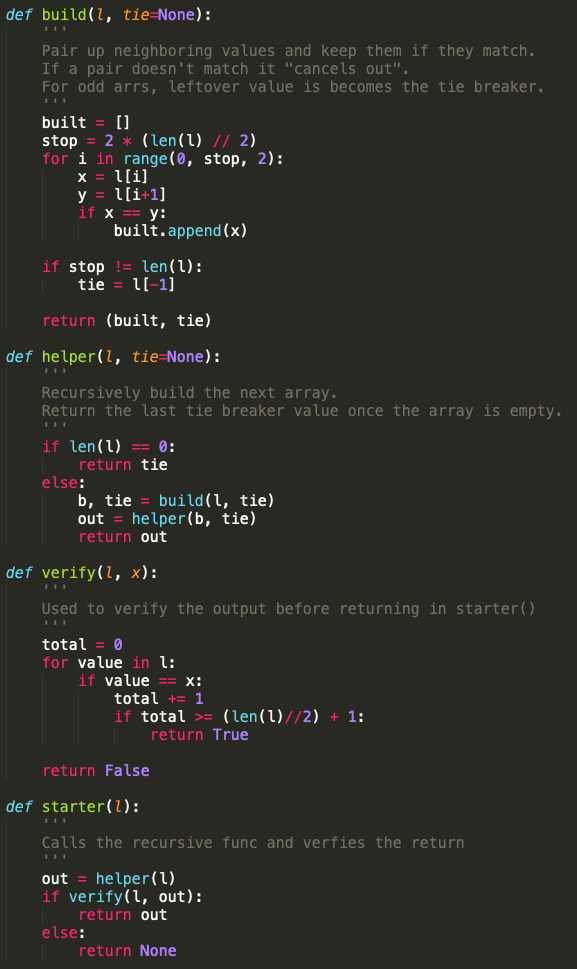
\includegraphics[scale=0.4]{majority_code.png}


\subsection*{Explanation}
The algorithm makes pairs through the list. Any pairs that match get passed down to the array for the next recursion. Non-matching pairs "cancel" eachother's votes out and are removed. For odd-length lists the leftover entry becomes a tie-breaker value. Once the function receives an empty array it will return the tie-breaker value, after verifying the value by counting the number of occurrences in the original array. 

\subsection*{Runtime}
General runtime for this algo:\\
$T(n) = T(n/2) + O(n)$\\

\noindent For the master theorem, the values are:\\
\noindent $\alpha=1$: because each call of the function results in one recursive call.\\
$\beta=2$: because the size of the array for each next call will be at most of size $n/2$\\
$\gamma=1$: because the work of verifying the solution is $O(n)$, meaning for $O(n^\gamma)$, $\gamma = 1$\\

\noindent In this case: $\gamma > \log_\beta \alpha$ $(1 > \log_2 1)$\\
Therefore this algorithm has: $O(n^\gamma$) or $O(n)$.

\newpage
\section*{Problem-3 (30 points)}
Design an algorithm to multiply any $n$-bit integer with any $m$-bit integer where $n \ge m$ in $O(n\, m^{\log_2(3) - 1})$ time.
 

\subsection*{Solution}

\begin{algorithm}
\caption{multiplySameSize($x, y$)}
\begin{algorithmic} 
\REQUIRE two $m$-bit sized integers
% \ENSURE $y = x^n$
\smallskip
\STATE $m \leftarrow$ bit size of $x$ (or $y$)

\smallskip
\STATE $x_l, x_r \leftarrow$ bits of $x$ split at $\floor{m/2}$
\STATE $y_l, y_r \leftarrow$ bits of $y$ split at $\floor{m/2}$

\smallskip
\STATE $a \leftarrow$ multiplySameSize($x_l, y_l$)
\STATE $b \leftarrow$ multiplySameSize($x_r, y_r$)
\STATE $c \leftarrow$ multiplySameSize($x_l + x_r, y_l + y_r$)

\smallskip
\RETURN $(a \cdot 2^x) + ((c-a-b) \cdot 2^{x/2}) + b$

\end{algorithmic}
\end{algorithm}


\begin{algorithm}
\caption{multiply($x, y$)}
\begin{algorithmic} 
\REQUIRE int $x$ with size $n$; int $y$ with size $m$ (where $n \geq m$)

\STATE $iters \leftarrow \lceil n/m \rceil$
\STATE zero-pad $x$ to be size: $m * iters$
\STATE $total \leftarrow 0$

\FOR{$j \in 0..iters$}
\STATE $x_j \leftarrow $ the $j$-th chunk of $m$ bits in $x$
\STATE $c \leftarrow $ multiplySameSize($x_j, y$)
\STATE $c \leftarrow c \cdot 2^{m \cdot j}$ (leftshift section to match original position in x)
\STATE $total \mathrel{{+}{=}} c$
\ENDFOR

\RETURN $total$

\end{algorithmic}
\end{algorithm}

\subsection*{Explanation}
A multiplication can be done using the multiplication of: the first halves of each number, second halves of each number, and sum of the halves for each number. The result can be found with the components and some addition/subtraction, as well as multiplication with powers of two (which can be easily done with left shifts). Once the function recursively halves the inputs down to 1-bit numbers, then multiplication can be done with a binary AND.\\
If the two numbers are different sizes then the second function multiply() can be used to split up the larger integer into chunks of the size of the smaller integer. If the larger integer doesn't cleanly divide into chunks with sizes of the smaller integer, then the larger integer can be zero-padded to make it large enough do divide cleanly.

\subsection*{Runtime}
General process for this multiplySameSize() involves:\\
$T(n) = 3T(n/2) + O(1)$

\bigskip \noindent Master theorem application for multiplySameSize():\\
$\alpha=3$: because each call of the multiply function will result in 3 recursive sub-calls.\\
$\beta=2$: $n$ will be reduced to $n/2$ for subcalls of multiplySameSize().\\
$\gamma=0$: because the work to combine sub calls will be a constant runtime process (the additions/multiplications for the second return line). $O(n^\gamma)=O(1)$ requires $\gamma=0$.

\medskip \noindent In this case: $\gamma < \log_\beta \alpha$ ($0 < \log_2 3$), therefore multiplySameSize() has $O(m^{\log_2 3})$, where $m$ is the bit-size of $x$ and $y$.\\
During the algorithm, multiply() will call multipySameSize() at least $\lceil n/m \rceil$ times. Therefore multiply() has $O((n/m) \cdot m^{\log_2 3})$ or $O(nm^{\log_2 3 - 1})$.

\end{document}